\chapter{Introduction}
\label{chap1}
Ever since the paper shredder was invented, people have worked on sticking the pieces back together again. Recently, techniques permitting the purely electronic storage and transmittal of sensitive documents have been developed but, because of convenience or for legal reasons, many sensitive documents are still printed and eventually shredded. Traditionally, the cost of reconstructing these documents was considered prohibitive(though there have been cases where such a steep cost could be justified \ref{fig:iranDoc}), however with the development of methods that partly automate the process this situation is changing. \\ It is currently unclear what level of security the paper shredder still offers.

\begin{figure}[h]
    \centering
    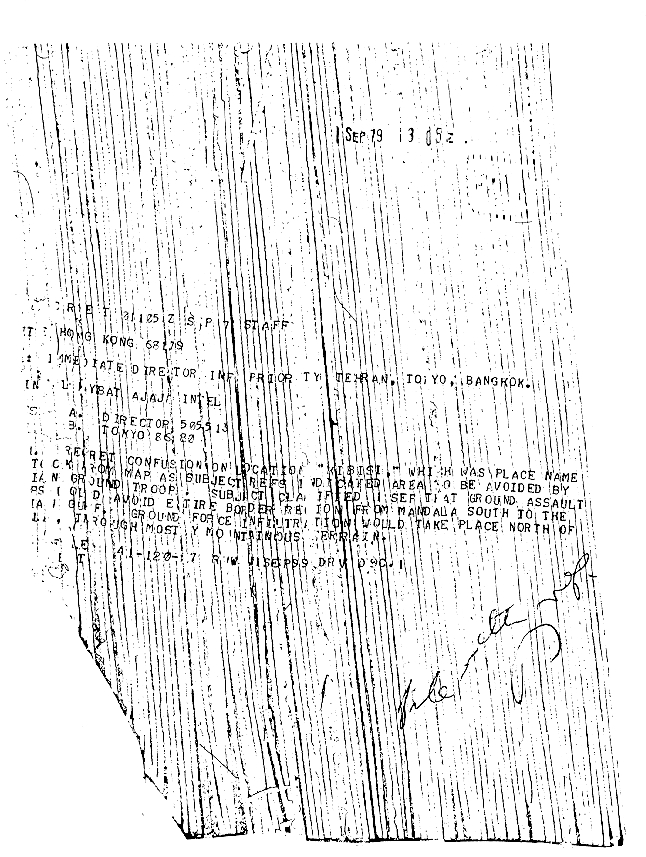
\includegraphics[width=0.5\textwidth, height=9cm]{iran}
    \caption{A shredded document belonging to the CIA. This was reconstructed by a team of carpet weavers during the 1979 Iran hostage crisis. The reconstructed documents were eventually released by the Iranian government in a series of books \cite{P10}}
    \label{fig:iranDoc}
\end{figure}

\section{Importance}
Techniques such as dumpster diving have long been used to gain access to sensitive information. Skoudis \cite{P11}, for instance, discusses how such techniques, in conjunction with basic social engineering, can completely circumvent any security measures placed to protect a system. Similar approaches also account for part of the several million identity theft cases identified by the US Federal Trade Commission every year \cite{P12}. In the face of this danger, both Skoudis and the Federal Trade Commission identify the shredding of sensitive documents as a good security measure to take. \cite{P11, P13}. However, the development of commercial shredded document reconstruction software \cite{P14} casts doubts on the benefit of shredding sensitive documents and highlights the need for further research in this area.
 
One recent initiative looking at the reconstruction problem was the 2011 DARPA\footnote{Defense Advanced Research Projects Agency} shredding challenge, which offered a \$50,000 prize for the first team to successfully solve a series of  puzzles printed on 5 shredded documents.\cite{P15} The puzzle was solved in 32 days, with the winning team managing to reconstruct a total of 5 documents shredded into more than 10,000 pieces. \ref{fig:darpa}

The DARPA Challenge was motivated by the difficulties that troops encounter in war zones while trying to make sense of the remnants of destroyed documents. Further research in this area could  have a significant impact on a number of related problems in the fields of forensics and investigative science. One of the most notable projects that could benefit from advancements in unshredding technology is the  current effort to recover the shredded archives of the East German secret police. The STASI\footnote{The Ministry for State Security - The official state security service of East Germany} destroyed most of its archives before the 1990 reunification with West Germany. These archives consist of 16,000 bags of shredded documents and, so far, it has taken three dozen people six years to reconstruct 300 of them.\cite{P16} At that rate, it would take 11,520 person-years to finish the task. \ref{fig:stasi}

\begin{figure}[H]
    \centering
    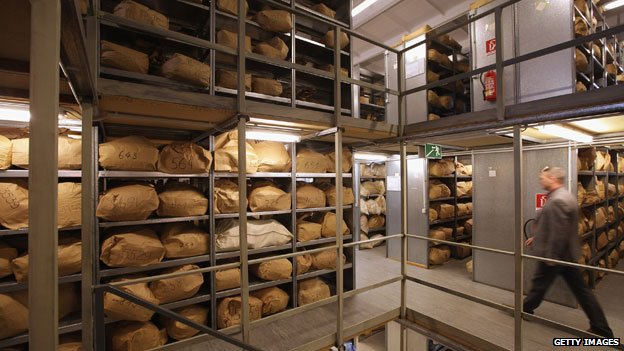
\includegraphics[width=0.9\textwidth, height=6.5cm]{stasi}
    \caption{A fraction of the 16,000 bags containing the shredded STASI archives.}
    \label{fig:stasi}
\end{figure}

\begin{figure}[H]
    \centering
    \begin{subfigure}[b]{\textwidth}
        \centering
        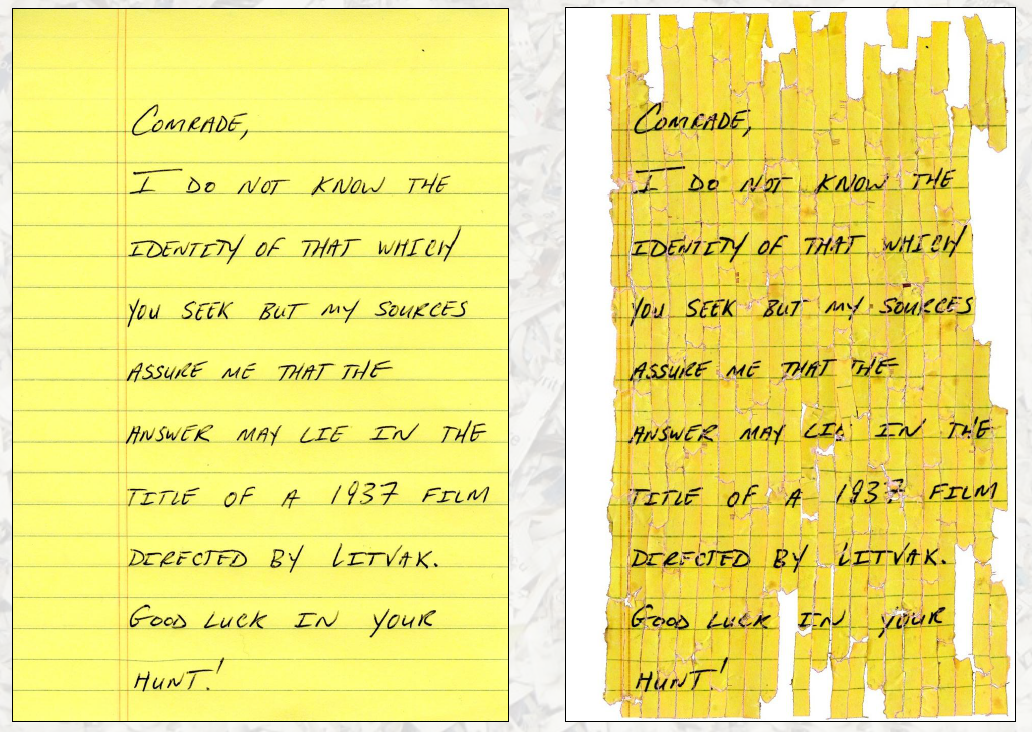
\includegraphics[width=\textwidth]{darpa1}
        \caption{One of the easiest documents in the DARPA Challenge. It is perfectly reconstructed.}
    \end{subfigure}
    ~
    \begin{subfigure}[b]{\textwidth}
        \centering
        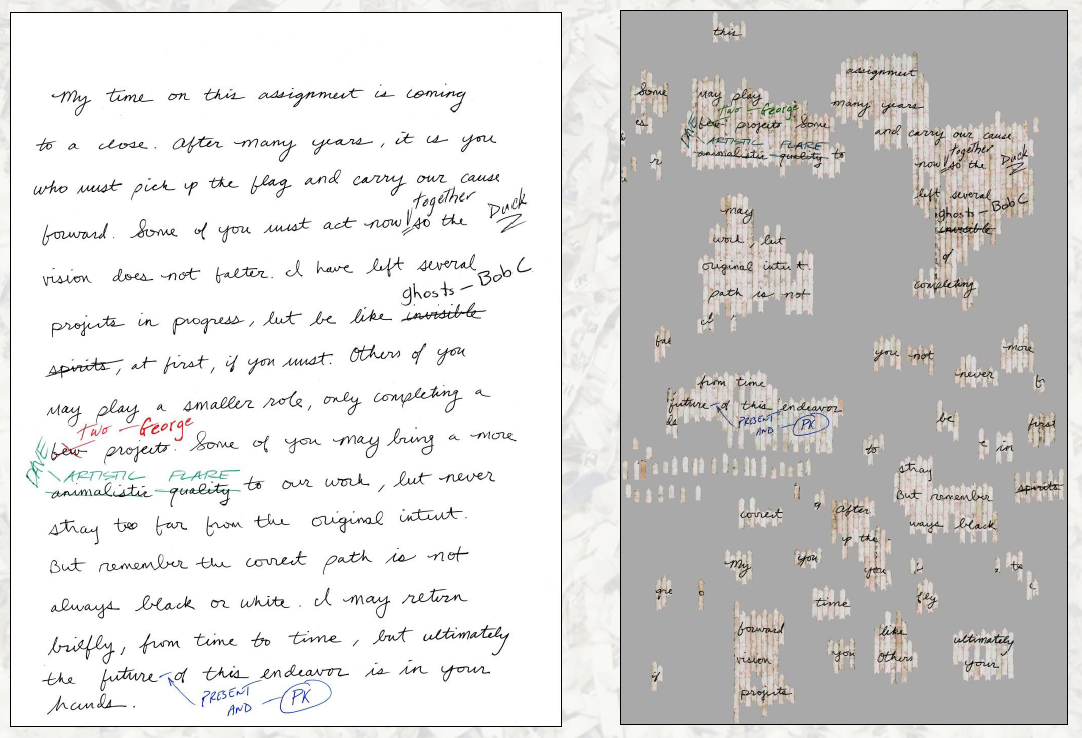
\includegraphics[width=\textwidth]{darpa4}
        \caption{One of the hardest documents in the DARPA Challenge. Even though the reconstruction is far from complete, the competitors were able to extract the information they needed from this partial solution.}
    \end{subfigure}
     \caption{Two of the DARPA Challenge documents \cite{P15}}
    \label{fig:darpa}
\end{figure}


\section{Paper Shredders}
Paper shredders come in many different shapes, sizes and price ranges. It is therefore worthwile to take a closer look at the types of shredders in use and at the security they offer. \\
There are 3 main types of shredders:
\begin{itemize}
\item {\bf Strip-cut:} The cheapeast and most common variant. The paper is cut in long vertical strips. The width of the strips varies with the model.
\item {\bf Cross-cut:} The type of shredder typically used when extra security is deemed necessary. The paper is cut both vertically and horizontally into small rectangles. The size of the rectangles again varies with the model.
\item {\bf Other:} There are several types of industrial or specialist shredders that fall outside of the above categories. These include things such as \emph{Grinders} which consist of a rotating shaft with blades that grinds the paper untill it is small enough to fall through a mesh. These types of shredders are rarely used outside of industrial settings, so we shall not consider them further.
\end{itemize}

The strip and cross-cut shredders can be further classified according to the DIN\footnote{Deutsche Industrial Norm} 32757 standard which are used throughout Europe. \cite{P16} This standard defines 6 common categories of strip or cross-cut shredders based on the level of security they offer.\ref{tab:din}

\begin{table}[h]
  \centering
  \begin{tabular}{lllll}
    \toprule
    \multirow{2}{*}{Security Level} & \multicolumn{2}{l}{Strip-Cut} & \multicolumn{2}{l}{Cross-Cut} \\
    \cmidrule(r){2-3} 
    \cmidrule(r){4-5}
    & Shred size & No. shreds/page & Shred size & No. shreds/page \\
    Level 1 & 12 mm. & 18 & 11x40 mm. & 152 \\
    Level 2 & 6 mm. & 35 & 8x40 mm. & 216 \\
    Level 3 & 2 mm. & 105 & 4x30 mm. & 530 \\
    Level 4 & N.A. & N.A. & 2x15 mm. & 2100 \\
    Level 5 & N.A. & N.A. & 0.8x12 mm. & 6575 \\
    Level 6 & N.A. & N.A. & 0.8x4 mm. & 19725 \\
    \bottomrule
  \end{tabular}
  \caption{Levels of security defined by the DIN 32757 standard}
  \label{tab:din}
\end{table}

In order to get a better intuitive sense of these, we can look at some some shreds outputed by machines at each level \ref{fig:dinOut}

\begin{figure}[h]
        \centering
        \begin{subfigure}[b]{0.15\textwidth}
                \centering
                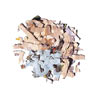
\includegraphics[width=\textwidth]{securitylevel1}
                \caption{Level 1}
        \end{subfigure}
        ~ 
        \begin{subfigure}[b]{0.15\textwidth}
                \centering
                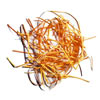
\includegraphics[width=\textwidth]{securitylevel2}
                \caption{Level 2}
        \end{subfigure}
        ~ 
        \begin{subfigure}[b]{0.15\textwidth}
                \centering
                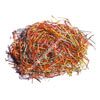
\includegraphics[width=\textwidth]{securitylevel3}
                \caption{Level 3}
        \end{subfigure}
        ~ 
        \begin{subfigure}[b]{0.15\textwidth}
                \centering
                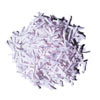
\includegraphics[width=\textwidth]{securitylevel4}
                \caption{Level 4}
        \end{subfigure}
        ~ 
        \begin{subfigure}[b]{0.15\textwidth}
                \centering
                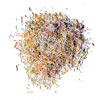
\includegraphics[width=\textwidth]{securitylevel5}
                \caption{Level 5}
        \end{subfigure}
        ~ 
        \begin{subfigure}[b]{0.15\textwidth}
                \centering
                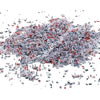
\includegraphics[width=\textwidth]{securitylevel6}
                \caption{Level 6}
        \end{subfigure}
        \caption{The output generated by shredders at the different DIN levels.\cite{P16} }
        \label{fig:dinOut}
\end{figure}

As can be seen, the ammount of security offered varies drastically. At level 1 the paper could feasibly be reasembled by hand, while at level 6, the noise introduced by the cutting and scanning of the pieces would likely make a full reconstruction impossible.

\section{Roadmap}

In Chapter \ref{chap2} we formally defined the problem being analyzed, specify any simplifying assumptions and look at its complexity and how it can be divided into subproblems. In Chapter \ref{chap3} we look at previously published related work. In Chapter \ref{chap4} a novel probabilistic score function is proposed and shown to perform well in comparison with the standard cost functions used in literature. In Chapter \ref{chap5} several tractable search heuristics are analysed. \todo{Complete this section}
